\section{Protocol} \fxnote{Did we want to add something about asking them about the pain after each methods? or what did we discuss about this}
This protocol will describe the present study, which consist of two experiments testing pain tolerance and pain threshold after practicing mindfulness meditation or after not practicing mindfulness meditation. 

\subsection{Purpose}
The treatment of chronic pain has constraints, as the treatments are only relieving the pain instead of curing the pain. Another issue is that some of these treatments, example medication, have side effect, as described in \secref{sec:treatment}. 
There is alternative to medication such as yoga, hypnosis and physical therapy, psychological therapy and chiropractor, which have shown to have an influence on relieving pain. But these treatments are often used in combination with pharmaceutical treatment. Furthermore, most of these alternative require an external person to apply, which can result in high costs, as mention in \secref{sec:treatment}.
An alternative to the present treatment is mindfulness meditation, which have shown an effect on relieving conditions as stress, depression and  anxiety through the ability to enhance emotion regulation, cognitive control, acceptance and positive mood, as described in \secref{sec:SOTA}. 
Different studies have shown that practicing meditation have an effect on reliving pain. However, these studies have most often investigated long-term mindfulness meditation for patient with eater chronic pain or low back pain. There is a limit on studies that have investigated short-term in patient with neck pain, why this could be interesting to investigate further, as approximately 25\% of the chronic pain patients suffer from this condition. In order to investigated the influence of mindfulness meditation on pain threshold and pain tolerance for people with neck pain following hypothesis is proposed:
\vspace{-.5cm}
\begin{itemize}
\item Short-term mindfulness meditation increases the pressure pain threshold and the pressure pain tolerance.
\end{itemize}

\subsection{Subjects}
Forty healthy subjects were recruited for the experiment, 20 males (M) and 20 females (F) with a mean age $\pm$XX. A homogeneous group of participants were enrolled in order to limit the amount of variables in the study. For insuring this, specific inclusion and exclusion criteria have been formed for this experiment. 

\textbf{Inclusion criteria:}
\vspace{-.5cm}
\begin{itemize}
	\item Healthy subjects age between 20-30 years
	\vspace{-.3cm}
	\item Normal BMI (F: 19-24 M: 20-25)
	\vspace{-.3cm}
	\item Must have time to meditate for 5 days, 30 minutes per day.
\end{itemize}

\textbf{Exclusion criteria:}
\vspace{-.5cm}
\begin{itemize}
	\item Ongoing meditation practice 
	\vspace{-.3cm}
	\item Acute or chronic pain
	\vspace{-.3cm}
	\item Pregnancy 
	\vspace{-.3cm}
	\item Neurological, musculoskeletal or mental illness
	\vspace{-.3cm}
	\item Signs or symptoms of any serious systemic diseases 
	\vspace{-.3cm}
	\item Psychiatric, analgesic or other medications that might influence their response to pain 
		\vspace{-.3cm}
	\item Abusive drug or alcohol use
		\vspace{-.3cm}
	\item Lack of ability to cooperate
\end{itemize}

\vspace{-.5cm}
Furthermore, is it not necessary that subjects believe in the effect of mindfulness meditation.\fxnote{I don't know about this sentence, i think it does not fit in here. Maybe it is more something we should write for the participants or could we put it in as one of our criteria?.}

\subsection{Approach} 
For this particular experiment a parallel study was conducted. The subjects recruited for the experiment were randomly assigned in two different groups, the control group or the treatment group, with a equal amount of female and males in the groups. The control group consisted of twenty subjects no meditation. The treatment group consisted of twenty subjects meditation. The structure of the study design is illustrated on \figref{fig:studydesign}. 

\begin{figure}[H]
	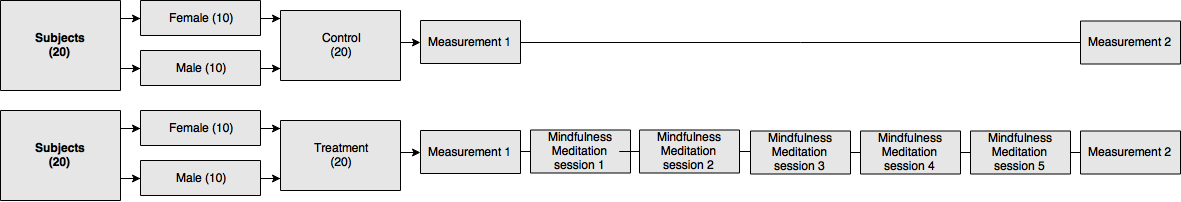
\includegraphics[width=1\textwidth]{figures/studydesign.png} 
	\caption{Parallel study design.}
	\label{fig:studydesign}  
\end{figure}  

There will be seven to eight days between the measurements. The treatments groups start practicing mindfulness meditation three or four days after the first measurement and will then practice mindfulness meditation for five days and will on the last day of meditation be measured again.

\subsection{Setup}
The Pressure Pain Threshold (PPT), defined as the pressure at which the sensation changed from pressure to pain, has been recognized as an effective and reliable way to quantify pain measures. In this study PPT was measured using Wagner Force Ten$^{TM}$ Digital force Gage. PPT were measured in the upper trapezius. Testing points were marked to ensure reliable and rapid location during the experimental procedure. 
The algometer was applied four times, two on the left side and two on the right side of the upper trapezius, and the average of the registrations was filed. The subjects had a 5 minutes resting time between measurements. PPT values were measured two times, the first day of the study and after 5 days since the first measure.

\subsubsection{Mindfulness meditation}
The treatment group should do guided meditation for 30 minutes in small groups for 5 days. On the first day the mediators would be giving a short introduction to mindfulness meditation. During the meditation the subjects would be in a sitting position with the face  away from the other subjects, to assure that they would not get distracted. 


\subsection{Procedure}

Control group
Treatment group


\subsubsection{Data Analysis}
To test the hypothesis statistical test was used.The choice of statistically test depends on the the distribution and variance of the dataset. Since, two groups are compared a t-test or Mann-Whitney depending on the distribution. If the data is normal distributed parametric a t-test will be used otherwise a the non-parametric test Mann-Whitney will be used. 